\section{Introduction}
\label{sec:intro}

%1. Why UQ is important for this problem?
%2. Challenges pertaining to UQ. Include a table for exponential scaling. 
%3. What has been done in previous UQ studies for atomistic level simulations.
%4. How we tried to address the challenge in our previous work.
%5. How is this work different?
%6. Key contributions.
%7. Organization of the paper.

Non-equilibrium molecular dynamics (NEMD) simulations are commonly used to investigate
bulk thermal conductivity of non-metallic elements such as carbon, silicon, and
germanium~\cite{Dumitrica:2010}. The system is subjected to either a heat flux or a temperature
gradient by means of thermostatting. The resulting steady-state temperature gradient in the
former and heat exchange between the thermostats in the latter is recorded. The thermal
conductivity at a given system size is then estimated using Fourier's law. In the
so-called direct method~\cite{Schelling:2002,Turney:2009,Zhou:2009,Landry:2009,
McGaughey:2006,Ni:2009,Shi:2009,Wang:2009,Papanikolaou:2008},
the thermal conductivity is estimated at multiple values of the
system size. The inverse of thermal conductivity ($\kappa^{-1}$) is plotted against the inverse of 
system size ($L^{-1}$) and a linear extrapolation procedure is used to estimate the y-intercept
of the plot. The inverse of the y-intercept is regarded as the bulk thermal conductivity
of the system since it corresponds to an infinitely large system (in theory). 

Although widely used, severe limitations are associated with the direct method.
The validity of the linear extrapolation procedure is not well established. Recent
investigations have revealed the existence of a non-linear trend in the $\kappa^{-1}$ vs. $L^{-1}$
relationship especially at large values of $L$ for Si~\cite{Sellan:2010}. Additionally, 
thermal conductivity estimate for a given size depends upon the choice of a potential
function and associated values of its parameters. Specifically for Si, the Stillinger-Weber (SW)
inter-atomic potential ($\Phi$) is commonly used in a large number of studies, as
%
\be
\Phi = \sum\limits_{i,j(i<j)}\phi_2(A,B,p,q,\alpha)\hspace{1mm}+\sum\limits_{i,j,k(i<j<k)}\phi_3(\lambda,\gamma)
\ee
%
However, according
to the methodology presented by Stillinger and Weber in~\cite{Stillinger:1985},
the following shortcomings must be noted:
%
\begin{itemize}
\item The SW potential function accounts for the second-order ($\phi_2$) and
third-order ($\phi_3$) atomic 
interactions. However, this representation can be inadequate in situations where 
higher order interactions become significant.  
\item Nominal values of the SW potential parameters were estimated using a 
limited search in a 7-dimensional parameter space. Regression-based parameter
estimates relied on the available set of experimental data while ensuring structural
stability. Hence, the estimates are tightly coupled with the set of data used for
calibration, and did not account for the presence of measurement uncertainty. 
\item Neither measurement error nor noise inherent in MD predictions (which can also be
significant) was accounted for in the analysis. 
\end{itemize}
%
Hence, using the same set of nominal values for a wide range of Si-based systems and
applications is not ideal. It is therefore important to estimate the SW parameter values
appropriate for a given application based on available data, and investigate the impact
of uncertainty in SW parameter values on NEMD predictions. 

This paper presents a computational framework aimed at dimension reduction
for enabling the forward problem of uncertainty propagation from the SW potential 
parameters to the quantity of interest (QoI) i.e. the bulk thermal conductivity of Si,
and the inverse problem of parameter estimation in a Bayesian setting using 
experimental data. For this purpose, we perform NEMD simulations of a Si bar
as discussed later in~\ref{sub:nemd}. The
motivation for input-space dimension reduction stems from exponential scaling in
computational effort with the number of parameters, illustrated in Table~\ref{tab:effort}. 
%
\newcommand{\ra}[1]{\renewcommand{\arraystretch}{#1}}
\begin{table}[htbp]
\centering
\ra{1.3}
\begin{tabular}{@{}ccc@{}}\toprule
Parameters & Model Runs & Time (1h/run)\\
\bottomrule
1 & 10 & 10 hours \\
2 & 10$^2$ & 4.2 days \\
3 & 10$^3$ & 1.4 months \\
4 & 10$^4$ & 1.2 years \\
5 & 10$^5$ & 11.6 years \\
6 & 10$^6$ & 115.7 years \\
7 & 10$^7$ & 1157.41 years \\
\bottomrule
\end{tabular}
\caption{Exponential scaling of computational effort with the number of uncertain parameters.}
\label{tab:effort}
\end{table}
%
Here, we consider that in order to perform uncertainty propagation,
an average of 10 runs along each input dimension
is needed, and each run takes approximately an hour. Therefore, the time required to 
perform the analysis in a 7-dimensional input space is $\mathcal{O}(10^3)$ years which makes it
intractable. Note that the considered compute times do not account for simulation queue times that further 
increase the time required for a run. 
Although computational gains can be realized using parallelism and sparse grids
for efficient surrogate construction~\cite{Bichon:2008,Ma:2009,Constantine:2012,Petvipusit:2014,Vohra:2014,Hu:2016}, 
the issue of exponential scaling would persist as long as the surrogate model is built in the original space of
the uncertain parameters.  
Hence, we aim to tackle the computational expense by focusing our efforts on reducing the 
dimensionality of the problem.
In our earlier effort, we presented a strategy~\cite{Vohra:2018b}
for constructing a surrogate for thermal conductivity dependence on the SW parameters
in a reduced space, evaluated using the derivative-based global sensitivity measures
(DGSMs)~\cite{Vohra:2018a}. The focus in that study was on determining the relative importance of the
parameters and fixing the unimportant parameters at their nominal values. In contrast, the
framework presented in this study aims to identify key directions in the input space along which the
QoI predominantly varies. The set of directions constitute the so-called 
\textit{active subspace}~\cite{Constantine:2015}.  

The active subspace methodology relies on estimating the partial derivative of the QoI 
with respect to each uncertain input. This requirement poses a couple of limitations on its
applicability: (1) The QoI is required to be differentiable in the considered input domain, and (2)
estimating the derivative typically requires additional model evaluations which
imposes a computational burden. Fortunately, in this case,
the thermal conductivity is observed to exhibit a smooth dependence on the SW parameters. 
To confirm this, we plot bulk thermal conductivity ($\kappa$) as a function of $\alpha$
and $\gamma$ in Figure~\ref{fig:kag} since it
predominantly varies along these directions, as discussed later
in Section~\ref{sec:results}. Note that the surface plot was generated using predictions from
the surrogate, constructed and verified for accuracy, also in Section~\ref{sec:results}.
The available set of 25 estimates using NEMD simulations are also shown. 
%
\begin{figure}[htbp]
\begin{center}
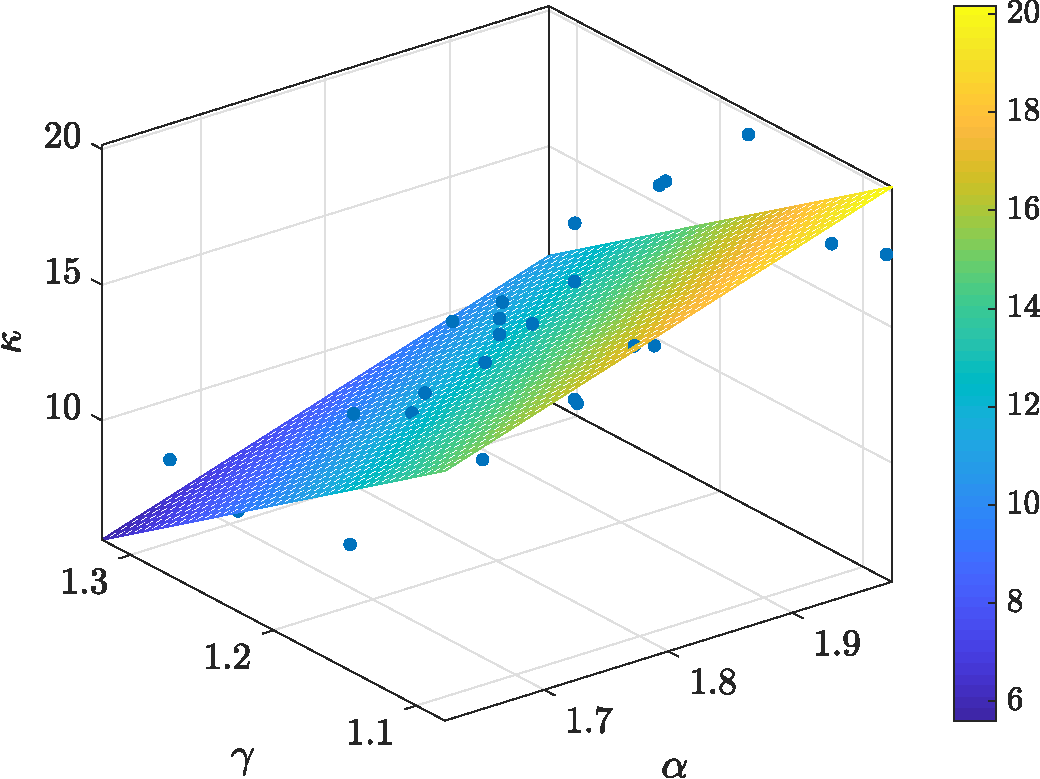
\includegraphics[width=0.45\textwidth]{./Figures/k_3D}
\caption{Variation of the bulk thermal conductivity of Si along the SW parameters, $\alpha$ 
and $\gamma$ in their respective intervals. The response surface is generated using predictions
of the surrogate, constructed later in Section~\ref{sec:results}. Individual predictions from NEMD
simulations are also plotted.}
\label{fig:kag}
\end{center}
\end{figure}
%
It is observed that the trends based on NEMD predictions are reasonably captured by
the response surface. Moreover, the variability in $\kappa$ is
observed to be quasi-linear as it ranges from roughly 6 to 20~W/m/K, and is  
differentiable in the considered intervals for $\alpha$ and $\gamma$.
Therefore, to mitigate the computational effort, we estimate the gradient
using a linear regression fit to the available set of model evaluations; as a result, we do not 
require additional atomistic evaluations at neighboring points as in the case of perturbation-based
derivative computation methods such as finite difference. We identify the active subspace
using the gradient information, and build a surrogate
model in the active subspace using a very small number of atomistic simulations
due to the reduced dimension. The active subspace-based surrogate model enables fast
uncertainty propagation and sensitivity analysis (forward problem) and Bayesian estimation
of SW parameters (inverse problem) due to the reduced dimensionality. 
The global sensitivity measures computed using the
active subspace are found to be consistent with earlier estimates 
based on Sobol' indices~\cite{Vohra:2018b}.

The remainder of this article is organized as follows. In Section~\ref{sec:bg}, we provide details
pertaining to the NEMD simulation, and a brief background on active subspaces.
The proposed computational framework for forward and inverse UQ is presented in
Section~\ref{sec:method}. Results based on implementing the framework to
compute the active subspace
are presented in Section~\ref{sec:results}. Finally, concluding remarks are provided 
in Section~\ref{sec:conc}.
































